% Generated from figures/generated/architecture.svg; do not hand edit.
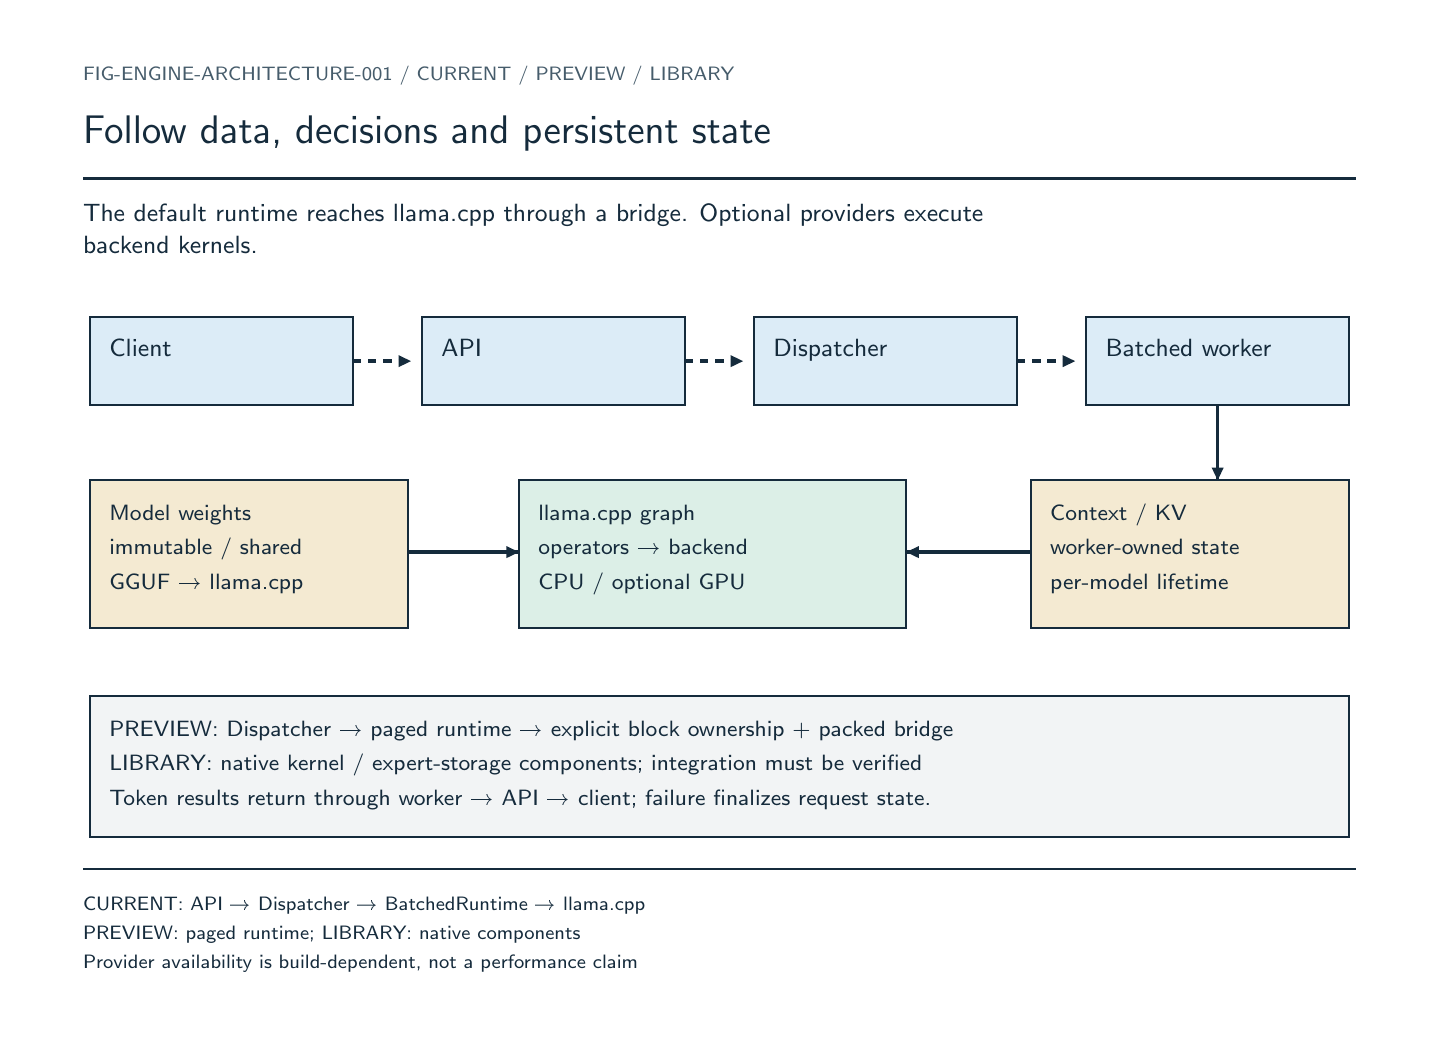
\begin{tikzpicture}[x=.5pt,y=-.5pt]
\path[use as bounding box] (0,0) rectangle (1000,720);
\path[fill=white,draw=none,line width=0.5pt] (0.0,0.0) rectangle (1000.0,720.0);
\node[inner sep=0pt,outer sep=0pt,anchor=base west,text={rgb,255:red,70;green,92;blue,107},font=\sffamily\fontsize{7.0}{8.4}\selectfont] at (40,38) {FIG-ENGINE-ARCHITECTURE-001  /  CURRENT / PREVIEW / LIBRARY};
\node[inner sep=0pt,outer sep=0pt,anchor=base west,text={rgb,255:red,21;green,43;blue,60},font=\sffamily\fontsize{15.0}{18.0}\selectfont] at (40,84) {Follow data, decisions and persistent state};
\draw[fill=none,draw={rgb,255:red,21;green,43;blue,60},line width=0.75pt] (40,109) -- (960,109);
\node[inner sep=0pt,outer sep=0pt,anchor=base west,text={rgb,255:red,21;green,43;blue,60},font=\sffamily\fontsize{9.5}{11.4}\selectfont] at (40,140) {The default runtime reaches llama.cpp through a bridge. Optional providers execute};
\node[inner sep=0pt,outer sep=0pt,anchor=base west,text={rgb,255:red,21;green,43;blue,60},font=\sffamily\fontsize{9.5}{11.4}\selectfont] at (40,163) {backend kernels.};
\path[fill={rgb,255:red,220;green,236;blue,247},draw={rgb,255:red,21;green,43;blue,60},line width=0.7pt] (45.0,209.0) rectangle (235.0,273.0);
\node[inner sep=0pt,outer sep=0pt,anchor=base west,text={rgb,255:red,21;green,43;blue,60},font=\sffamily\fontsize{9.0}{10.799999999999999}\selectfont] at (59,238) {Client};
\draw[fill=none,draw={rgb,255:red,21;green,43;blue,60},line width=1.25pt,dash pattern=on 3.0pt off 2.5pt] (235,241) -- (277,241);
\path[fill={rgb,255:red,21;green,43;blue,60},draw=none,line width=0.5pt] (277.00,241.00) -- (268.00,245.35) -- (268.00,236.65) -- cycle;
\path[fill={rgb,255:red,220;green,236;blue,247},draw={rgb,255:red,21;green,43;blue,60},line width=0.7pt] (285.0,209.0) rectangle (475.0,273.0);
\node[inner sep=0pt,outer sep=0pt,anchor=base west,text={rgb,255:red,21;green,43;blue,60},font=\sffamily\fontsize{9.0}{10.799999999999999}\selectfont] at (299,238) {API};
\draw[fill=none,draw={rgb,255:red,21;green,43;blue,60},line width=1.25pt,dash pattern=on 3.0pt off 2.5pt] (475,241) -- (517,241);
\path[fill={rgb,255:red,21;green,43;blue,60},draw=none,line width=0.5pt] (517.00,241.00) -- (508.00,245.35) -- (508.00,236.65) -- cycle;
\path[fill={rgb,255:red,220;green,236;blue,247},draw={rgb,255:red,21;green,43;blue,60},line width=0.7pt] (525.0,209.0) rectangle (715.0,273.0);
\node[inner sep=0pt,outer sep=0pt,anchor=base west,text={rgb,255:red,21;green,43;blue,60},font=\sffamily\fontsize{9.0}{10.799999999999999}\selectfont] at (539,238) {Dispatcher};
\draw[fill=none,draw={rgb,255:red,21;green,43;blue,60},line width=1.25pt,dash pattern=on 3.0pt off 2.5pt] (715,241) -- (757,241);
\path[fill={rgb,255:red,21;green,43;blue,60},draw=none,line width=0.5pt] (757.00,241.00) -- (748.00,245.35) -- (748.00,236.65) -- cycle;
\path[fill={rgb,255:red,220;green,236;blue,247},draw={rgb,255:red,21;green,43;blue,60},line width=0.7pt] (765.0,209.0) rectangle (955.0,273.0);
\node[inner sep=0pt,outer sep=0pt,anchor=base west,text={rgb,255:red,21;green,43;blue,60},font=\sffamily\fontsize{9.0}{10.799999999999999}\selectfont] at (779,238) {Batched worker};
\path[fill={rgb,255:red,244;green,234;blue,210},draw={rgb,255:red,21;green,43;blue,60},line width=0.7pt] (45.0,327.0) rectangle (275.0,434.0);
\node[inner sep=0pt,outer sep=0pt,anchor=base west,text={rgb,255:red,21;green,43;blue,60},font=\sffamily\fontsize{8.5}{10.2}\selectfont] at (59,356) {Model weights};
\node[inner sep=0pt,outer sep=0pt,anchor=base west,text={rgb,255:red,21;green,43;blue,60},font=\sffamily\fontsize{8.5}{10.2}\selectfont] at (59,381) {immutable / shared};
\node[inner sep=0pt,outer sep=0pt,anchor=base west,text={rgb,255:red,21;green,43;blue,60},font=\sffamily\fontsize{8.5}{10.2}\selectfont] at (59,406) {GGUF → llama.cpp};
\path[fill={rgb,255:red,220;green,239;blue,231},draw={rgb,255:red,21;green,43;blue,60},line width=0.7pt] (355.0,327.0) rectangle (635.0,434.0);
\node[inner sep=0pt,outer sep=0pt,anchor=base west,text={rgb,255:red,21;green,43;blue,60},font=\sffamily\fontsize{8.5}{10.2}\selectfont] at (369,356) {llama.cpp graph};
\node[inner sep=0pt,outer sep=0pt,anchor=base west,text={rgb,255:red,21;green,43;blue,60},font=\sffamily\fontsize{8.5}{10.2}\selectfont] at (369,381) {operators → backend};
\node[inner sep=0pt,outer sep=0pt,anchor=base west,text={rgb,255:red,21;green,43;blue,60},font=\sffamily\fontsize{8.5}{10.2}\selectfont] at (369,406) {CPU / optional GPU};
\path[fill={rgb,255:red,244;green,234;blue,210},draw={rgb,255:red,21;green,43;blue,60},line width=0.7pt] (725.0,327.0) rectangle (955.0,434.0);
\node[inner sep=0pt,outer sep=0pt,anchor=base west,text={rgb,255:red,21;green,43;blue,60},font=\sffamily\fontsize{8.5}{10.2}\selectfont] at (739,356) {Context / KV};
\node[inner sep=0pt,outer sep=0pt,anchor=base west,text={rgb,255:red,21;green,43;blue,60},font=\sffamily\fontsize{8.5}{10.2}\selectfont] at (739,381) {worker-owned state};
\node[inner sep=0pt,outer sep=0pt,anchor=base west,text={rgb,255:red,21;green,43;blue,60},font=\sffamily\fontsize{8.5}{10.2}\selectfont] at (739,406) {per-model lifetime};
\draw[fill=none,draw={rgb,255:red,21;green,43;blue,60},line width=1.25pt] (860,273) -- (860,327);
\path[fill={rgb,255:red,21;green,43;blue,60},draw=none,line width=0.5pt] (860.00,327.00) -- (855.65,318.00) -- (864.35,318.00) -- cycle;
\draw[fill=none,draw={rgb,255:red,21;green,43;blue,60},line width=1.25pt] (725,379) -- (635,379);
\path[fill={rgb,255:red,21;green,43;blue,60},draw=none,line width=0.5pt] (635.00,379.00) -- (644.00,374.65) -- (644.00,383.35) -- cycle;
\draw[fill=none,draw={rgb,255:red,21;green,43;blue,60},line width=1.25pt] (275,379) -- (355,379);
\path[fill={rgb,255:red,21;green,43;blue,60},draw=none,line width=0.5pt] (355.00,379.00) -- (346.00,383.35) -- (346.00,374.65) -- cycle;
\path[fill={rgb,255:red,242;green,244;blue,245},draw={rgb,255:red,21;green,43;blue,60},line width=0.7pt] (45.0,483.0) rectangle (955.0,585.0);
\node[inner sep=0pt,outer sep=0pt,anchor=base west,text={rgb,255:red,21;green,43;blue,60},font=\sffamily\fontsize{8.5}{10.2}\selectfont] at (59,512) {PREVIEW: Dispatcher → paged runtime → explicit block ownership + packed bridge};
\node[inner sep=0pt,outer sep=0pt,anchor=base west,text={rgb,255:red,21;green,43;blue,60},font=\sffamily\fontsize{8.5}{10.2}\selectfont] at (59,537) {LIBRARY: native kernel / expert-storage components; integration must be verified};
\node[inner sep=0pt,outer sep=0pt,anchor=base west,text={rgb,255:red,21;green,43;blue,60},font=\sffamily\fontsize{8.5}{10.2}\selectfont] at (59,562) {Token results return through worker → API → client; failure finalizes request state.};
\draw[fill=none,draw={rgb,255:red,21;green,43;blue,60},line width=0.75pt] (40,608) -- (960,608);
\node[inner sep=0pt,outer sep=0pt,anchor=base west,text={rgb,255:red,21;green,43;blue,60},font=\sffamily\fontsize{7.5}{9.0}\selectfont] at (40,638) {CURRENT: API → Dispatcher → BatchedRuntime → llama.cpp};
\node[inner sep=0pt,outer sep=0pt,anchor=base west,text={rgb,255:red,21;green,43;blue,60},font=\sffamily\fontsize{7.5}{9.0}\selectfont] at (40,659) {PREVIEW: paged runtime; LIBRARY: native components};
\node[inner sep=0pt,outer sep=0pt,anchor=base west,text={rgb,255:red,21;green,43;blue,60},font=\sffamily\fontsize{7.5}{9.0}\selectfont] at (40,680) {Provider availability is build-dependent, not a performance claim};
\end{tikzpicture}
